% \pagestyle{empty}
% \begin{center}
% \begin{figure}
% \centering%
% \vspace*{-3.5cm} \hspace*{-2.3cm} 
% 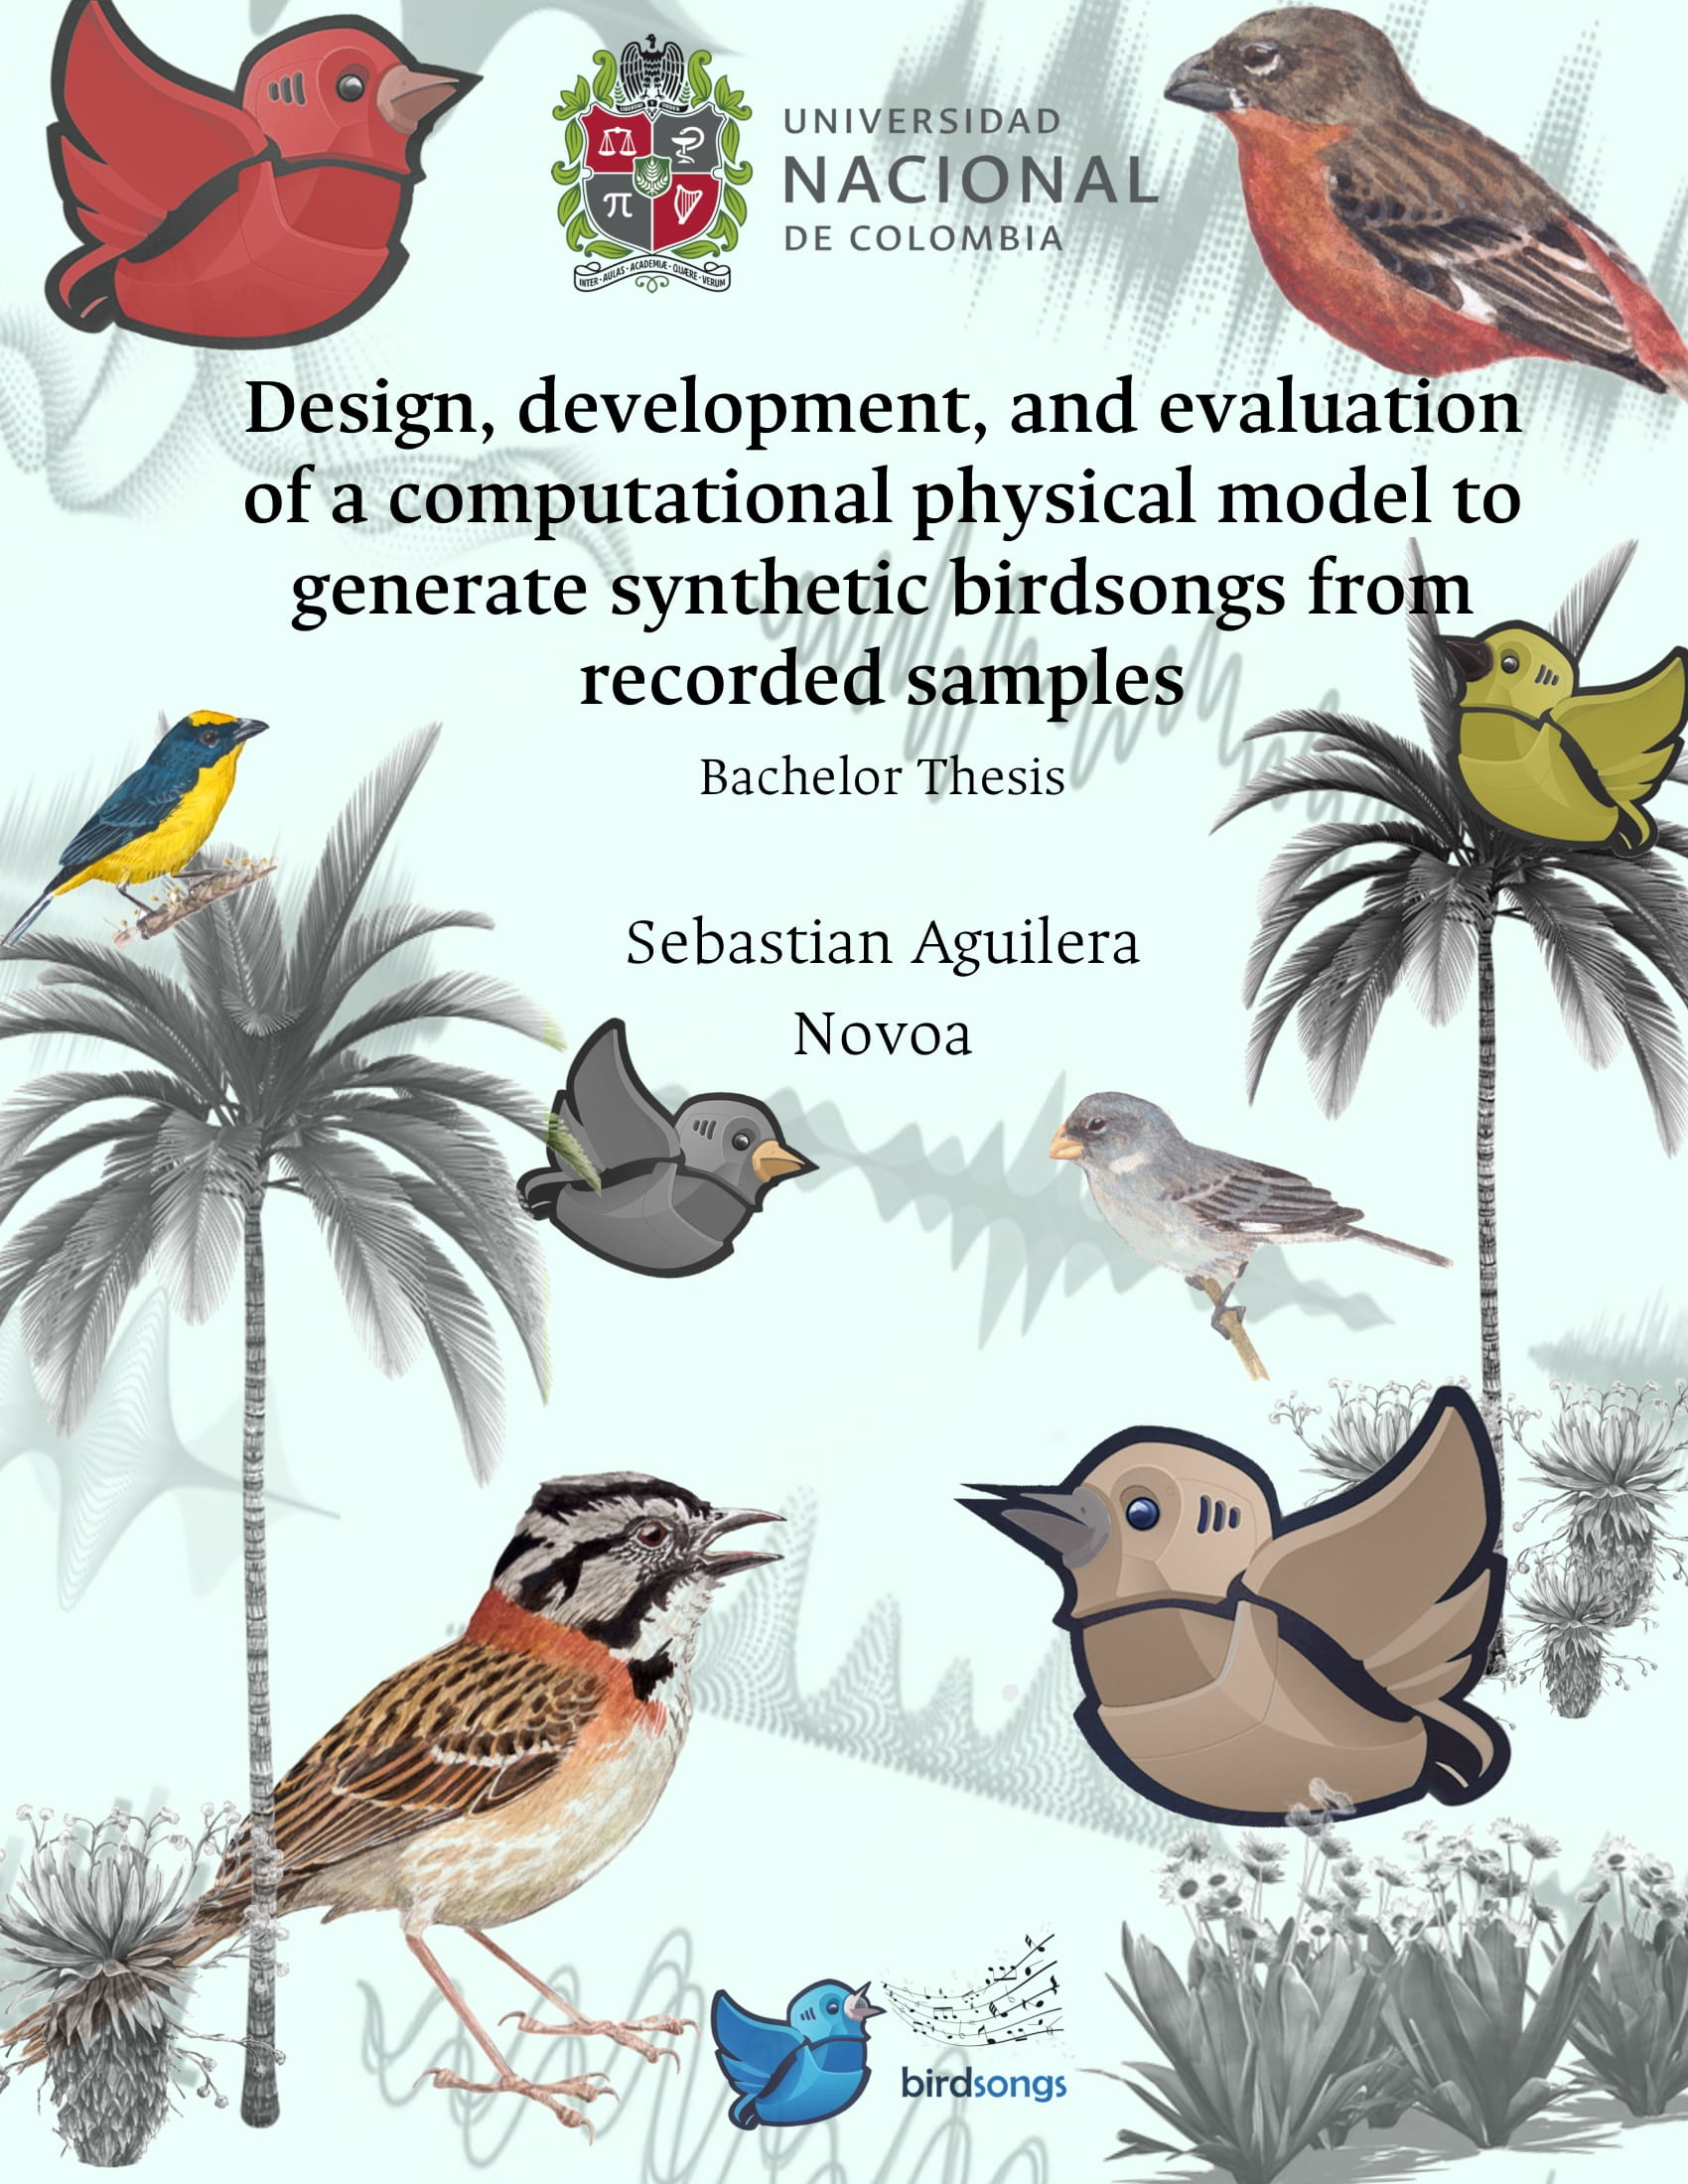
\includegraphics[width=1.3\linewidth]{Images/cover.png}
% \end{figure}
% \end{center}




\begingroup
\thispagestyle{empty}
\AddToShipoutPicture*{\put(0,0){\includegraphics[width=1.32  \linewidth]{Images/cover1.png}}} % Image background\centering
\centering
\vspace{0.4cm}\hspace{-3in}
\par\normalfont\fontsize{30}{30}\sffamily\selectfont
\textbf{Design, development, and
evaluation of a computational physical
model to generate synthetic birdsongs from recorded samples}\\
\centering
{\LARGE Bachelor Thesis}\par % Book title
\vspace*{1cm}
{\Huge Sebastian Aguilera\\Novoa}\par % Author name
\endgroup



\newpage
~\vfill
\thispagestyle{empty}

%\noindent Copyright \copyright\ 2014 Andrea Hidalgo\\ % Copyright notice

\noindent \textsc{Bachelor dissertation, National University of Colombia}\\

\noindent \href{https://github.com/saguileran/birdsongs}{\textsc{github.com/saguileran/birdsongs}}\\ % URL

\noindent This thesis was done under the supervision of professor Francisco Gómez Jaramillo, Datalab group leader. It is a requirement to obtain the degree in physics. \\ % License information

\noindent \textit{First release, December 2022} % Printing/edition date





\newpage{\pagestyle{empty}\clearpage}  %\cleardoublepage
\setcounter{page}{1}
\begin{center}
\begin{figure}
\centering%

\includegraphics[width=6.5cm]{Images/logo1.jpg}
\end{figure}
\thispagestyle{empty} \vspace*{1.0cm} \textbf{\huge
Diseño, desarrollo y evaluación de un modelo físico-computacional generador de cantos de aves sintéticos a
partir de cantos grabados.}\\[4.0cm]
\Large\textbf{Sebastian Aguilera Novoa}\\[4.0cm]
\small Universidad Nacional de Colombia\\
Facultad de Física, Departamento de Ciencias Naturales.\\
Bogotá, Colombia\\
2022\\
\end{center}

%\newpage{\pagestyle{empty}\cleardoublepage}

\newpage
\begin{center}
\thispagestyle{empty} \vspace*{0cm} \textbf{\huge
Design, development, and evaluation of a computational-physical model to generate synthetic birdsongs from recorded samples}\\[3.0cm]
\Large\textbf{Sebastian Aguilera Novoa}\\[3.0cm]
\small Degree work presented as a partial requirement for the PHYSICS degree:\\
\textbf{Bachelors in Physics}\\[2.5cm]
Director:\\
Francisco Gómez Jaramillo Ph.D.\\[4.5cm] 

National University of Colombia\\
Physics Faculty, Exact Science Department.\\
Bogotá, Colombia\\
2022\\
\end{center}

%\newpage{\pagestyle{empty}\cleardoublepage}

\newpage
\thispagestyle{empty} \textbf{}\normalsize
\\\\\\%

\begin{flushright}
\begin{minipage}{8cm}
    \noindent
        \small
        %\textit{"The voice of beauty speaks softly; it creeps only into the most fully awakened souls”} 
        \textit{In honor of my mother, because she was the giant shoulders that allowed me to be a scientist. \\ \\
        "Education is the most powerful weapon you can use to change the world."\\
        \hspace*{\fill}  Nelson Mandela}\\
%- Friedrich Nietzsche
\end{minipage}
\end{flushright}

\newpage
\thispagestyle{empty} \textbf{}\normalsize
\\\\\\%
\textbf{\LARGE Acknowledgment}
\addcontentsline{toc}{chapter}{Acknowledgment}\\\\

I want to thanks all the teaching staff of the Universidad Nacional de Colombia, who guided me to achieve my dreams. Professor Francisco Gomez for being a great educator and teach me the tools and knowledge to carry out this work, Professor Jorge Ruiz for teaching me all the ideas of numerical optimization; to Juan Ulloa, for our discussion and his advices that guide me to formulate and define the problem presented; and Professor Gabo Mindlin for always answering my questions about the  physics of the model and give me great advices. \\

I also want to thank all the my classmates and  friends to support me in this adventure: to Jonnatan, for his life teachings and for showing me the meaning and importance of friendship; to Sami, for sharing and brightening up several years of my life with their company letting me know what it is to be loved; to all the Miguels with whom I shared, discussed and they teach me many things; to Raul for being the best high school professor and for always giving me encouragement to study; and of course, to all the Sebastians I have met along this adventure and who make me love my name. I would like to thank all those who get involved in this adventure and share their time with me, I will keep you in my mind and my heart.\\  

%falta la ancina
Finally, I would also like to thank my father, for letting me be, and my brother, because his love for music went beyond the walls and splashed me, to both of them thanks for always being by my side and supporting my ideas and projects. And a special thank to my mother, for giving me life and the curiosity to live it, for supporting my education and showing me the beauty of life, because without her none of these will be possible.\\

Mother, thank you very much for making my dreams possible.

\newpage{\pagestyle{empty}\cleardoublepage}

\newpage


\textbf{\LARGE Abstract}\\

Any Colombian has probably heard a birdsongs at one time or another. In fact, Colombia is the country with the largest bird population in the world playing an important role in the conservation of bird, since the  richness of bird in an ecosystem will give information about the loss biodiversity and the sustainable of the ecosystem. As a physicist, I have been interested in how to use physical models to generate realistic data, especially in acoustic physics. I have studied how to simulate the production of sound by means of the means of the acoustics of musical instruments and the sound production of birds. However, musical acoustics are widely researched, as well the classification and identification of birds using their birdsongs, but the production of birdsongs is another matter. The best and most complete physical model that explains the production of sound in birds is the \textbf{motor gestures}\cite{simple_motor_gestures_2001} model, developed two decades ago i the Dynamical Systems Lab by professor G. Mindlin, which uses nonlinear ordinary differential equations to model  the organs involved in the production of sound in birds: \textbf{syrinx}\footnote{Main character for the sound production. A tissue that vibrates causing the air oscillates and modulate a sound pressure input to the trachea}, trachea, glottis, oro-oesophageal cavity (OEC), and beak. For his purpose, a control problem of two parameters, air sac pressure from the bird bronchi and labial tension, is formulated such that it generates a synthetic sample from simple paths of the parameters space and recorded birdsongs.\\

The present work designs, develops and evaluates a python packing for the motor gestures model. Using current tools of signal processing, numerical optimization, and object programming oriented, the model is successfully implemented making it fast of reproduce and easier develop. With the presented model implementation, the sound production of birds can be broadly studied: the parameters space and their impact on the synthetic birdsong. This implementation makes it possible to create several samples of synthetic birdsongs, with a few python command lines, and compare them through their spectral characteristics. Teherefore, the model allows us to create as many not complex birdsongs, with a fundamental frequency well defined, as we want and by modifying the path in the space parameters (motor gesture). In addition, future applications will allow us to identify and classify the bird by its motor gesture. \\

The performance of the model is evaluated mainly with the birdsong syllables of the colored sparrow (zonotrichia capensis or copeton), since this is a familiar bird in Colombia, and its generalization is tested with other oscine birds\footnotemark{bird in the Passeri suborder are called oscines or birdsongs}: Mimus gilvus, Euphonia laniirostris, and Rhinocryptidae. The results show that the model generates comparable birdsong syllables when the input audio is of high sound quality, low nose level, and the pitch is well computed. in other cases the model does not generate a comparable birdsong and may give a diverse birdsong. \\

\textbf{\small Key Words:} birdsong, numerical-optimization, signal-processing.